\documentclass[a4paper]{article}
\usepackage[margin=3cm]{geometry}
\usepackage[french]{babel}
\usepackage[utf8]{inputenc}
\usepackage{amsmath}
\usepackage{graphicx}
\usepackage{schemabloc}
\usepackage[colorinlistoftodos]{todonotes}

\title{CSE - Asservissement en couple d'un moteur DC}

\author{Corentin Smith - Gabriel Samain}

\date{\today}

\begin{document}
\maketitle


\section{Préambule}

\subsection{Objectif}

L'objectif de ce TP est de réaliser l'asservissement en couple / courant d'un moteur DC, le but final étant de simuler un effort par l'axe du moteur.

\subsection{Théorie}

Les équations électromécaniques donnent : 
$$
\begin{cases}
C = k \cdot \Phi \cdot I \\
E = k \cdot \Phi \cdot \Omega
\end{cases}
$$

Le principe fondamental de la dynamique donne :
$$
J \frac{d\Omega}{dt} = Cm - Cr
$$


\section{Boucle d'asservissement}

On réalise une boucle d’asservissement en récupérant l’intensité dans le moteur à l’aide d’une résistance de shunt.

\subsection{Schéma}

\begin{center}
\begin{tikzpicture}
\sbEntree{E}
\sbComp{comp}{E}
\sbRelier[$U_c$]{E}{comp}
\sbBloc{hach}{Hacheur}{comp}
\sbRelier[$\epsilon$]{comp}{hach}
\sbBloc{reg}{Régulateur}{hach}
\sbRelier[$U_h$]{hach}{reg}
\sbBloc{mot}{Moteur}{reg}
\sbRelier[u]{reg}{mot}
\sbSortie{S}{mot}
\sbRelier[$I$]{mot}{S}
\sbDecaleNoeudy[4]{S}{E}
\sbBlocr{shunt}{Shunt}{E}
\sbRelieryx{mot-S}{shunt}
\sbRelierxy[$U_m$]{shunt}{comp}
\end{tikzpicture}
\end{center}

Les blocs assurent les fonctions suivantes :
\begin{description}
  \item[Hacheur] 	Transforme le signal $\epsilon$ en PWM grâce à un comparateur à hysterésis et un signal triangle
  \item[Régulateur] Duplique et inverse le signal précédent puis l'injecte dans un pont en H
  \item[Moteur] 	Le système à contrôler
  \item[Shunt] 		Une résistance de shunt permet de “lire le courant” sous forme de tension
\end{description}

\subsection{Schéma électrique}

\begin{figure}[h!]
\centering
	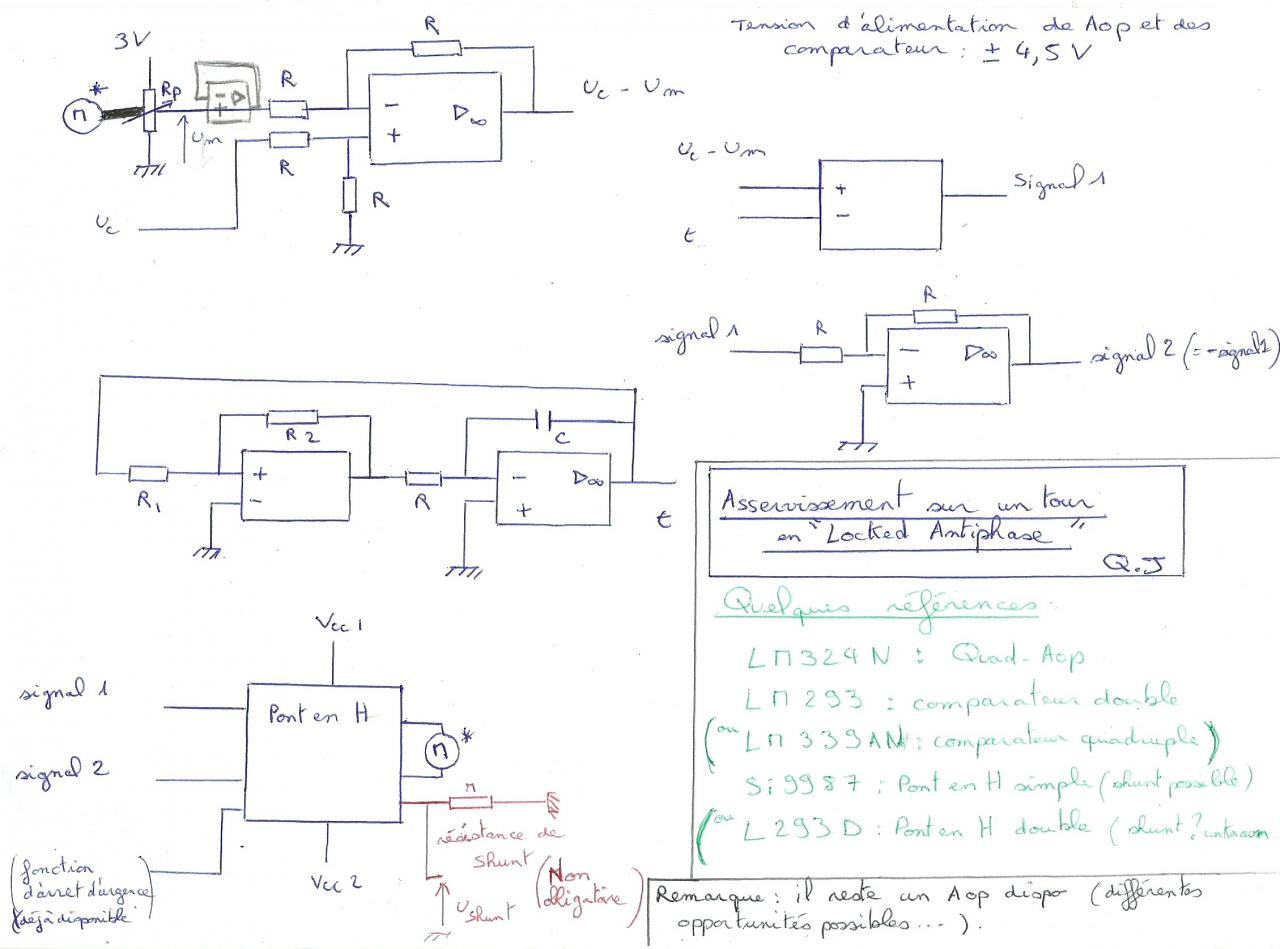
\includegraphics[width=1\textwidth]{schema}
	\caption{Schéma électrique}
\end{figure}


\subsection{Choix des composants}

\section{Réalisation}

\subsection{Simulation}

La simulation théorique du circuit se fait à l'aide du logiciel iCircuit qui permet une visualisation en temps réel des grandeurs physiques caractéristiques de chaque composant du circuit.
\begin{figure}
	\centering
	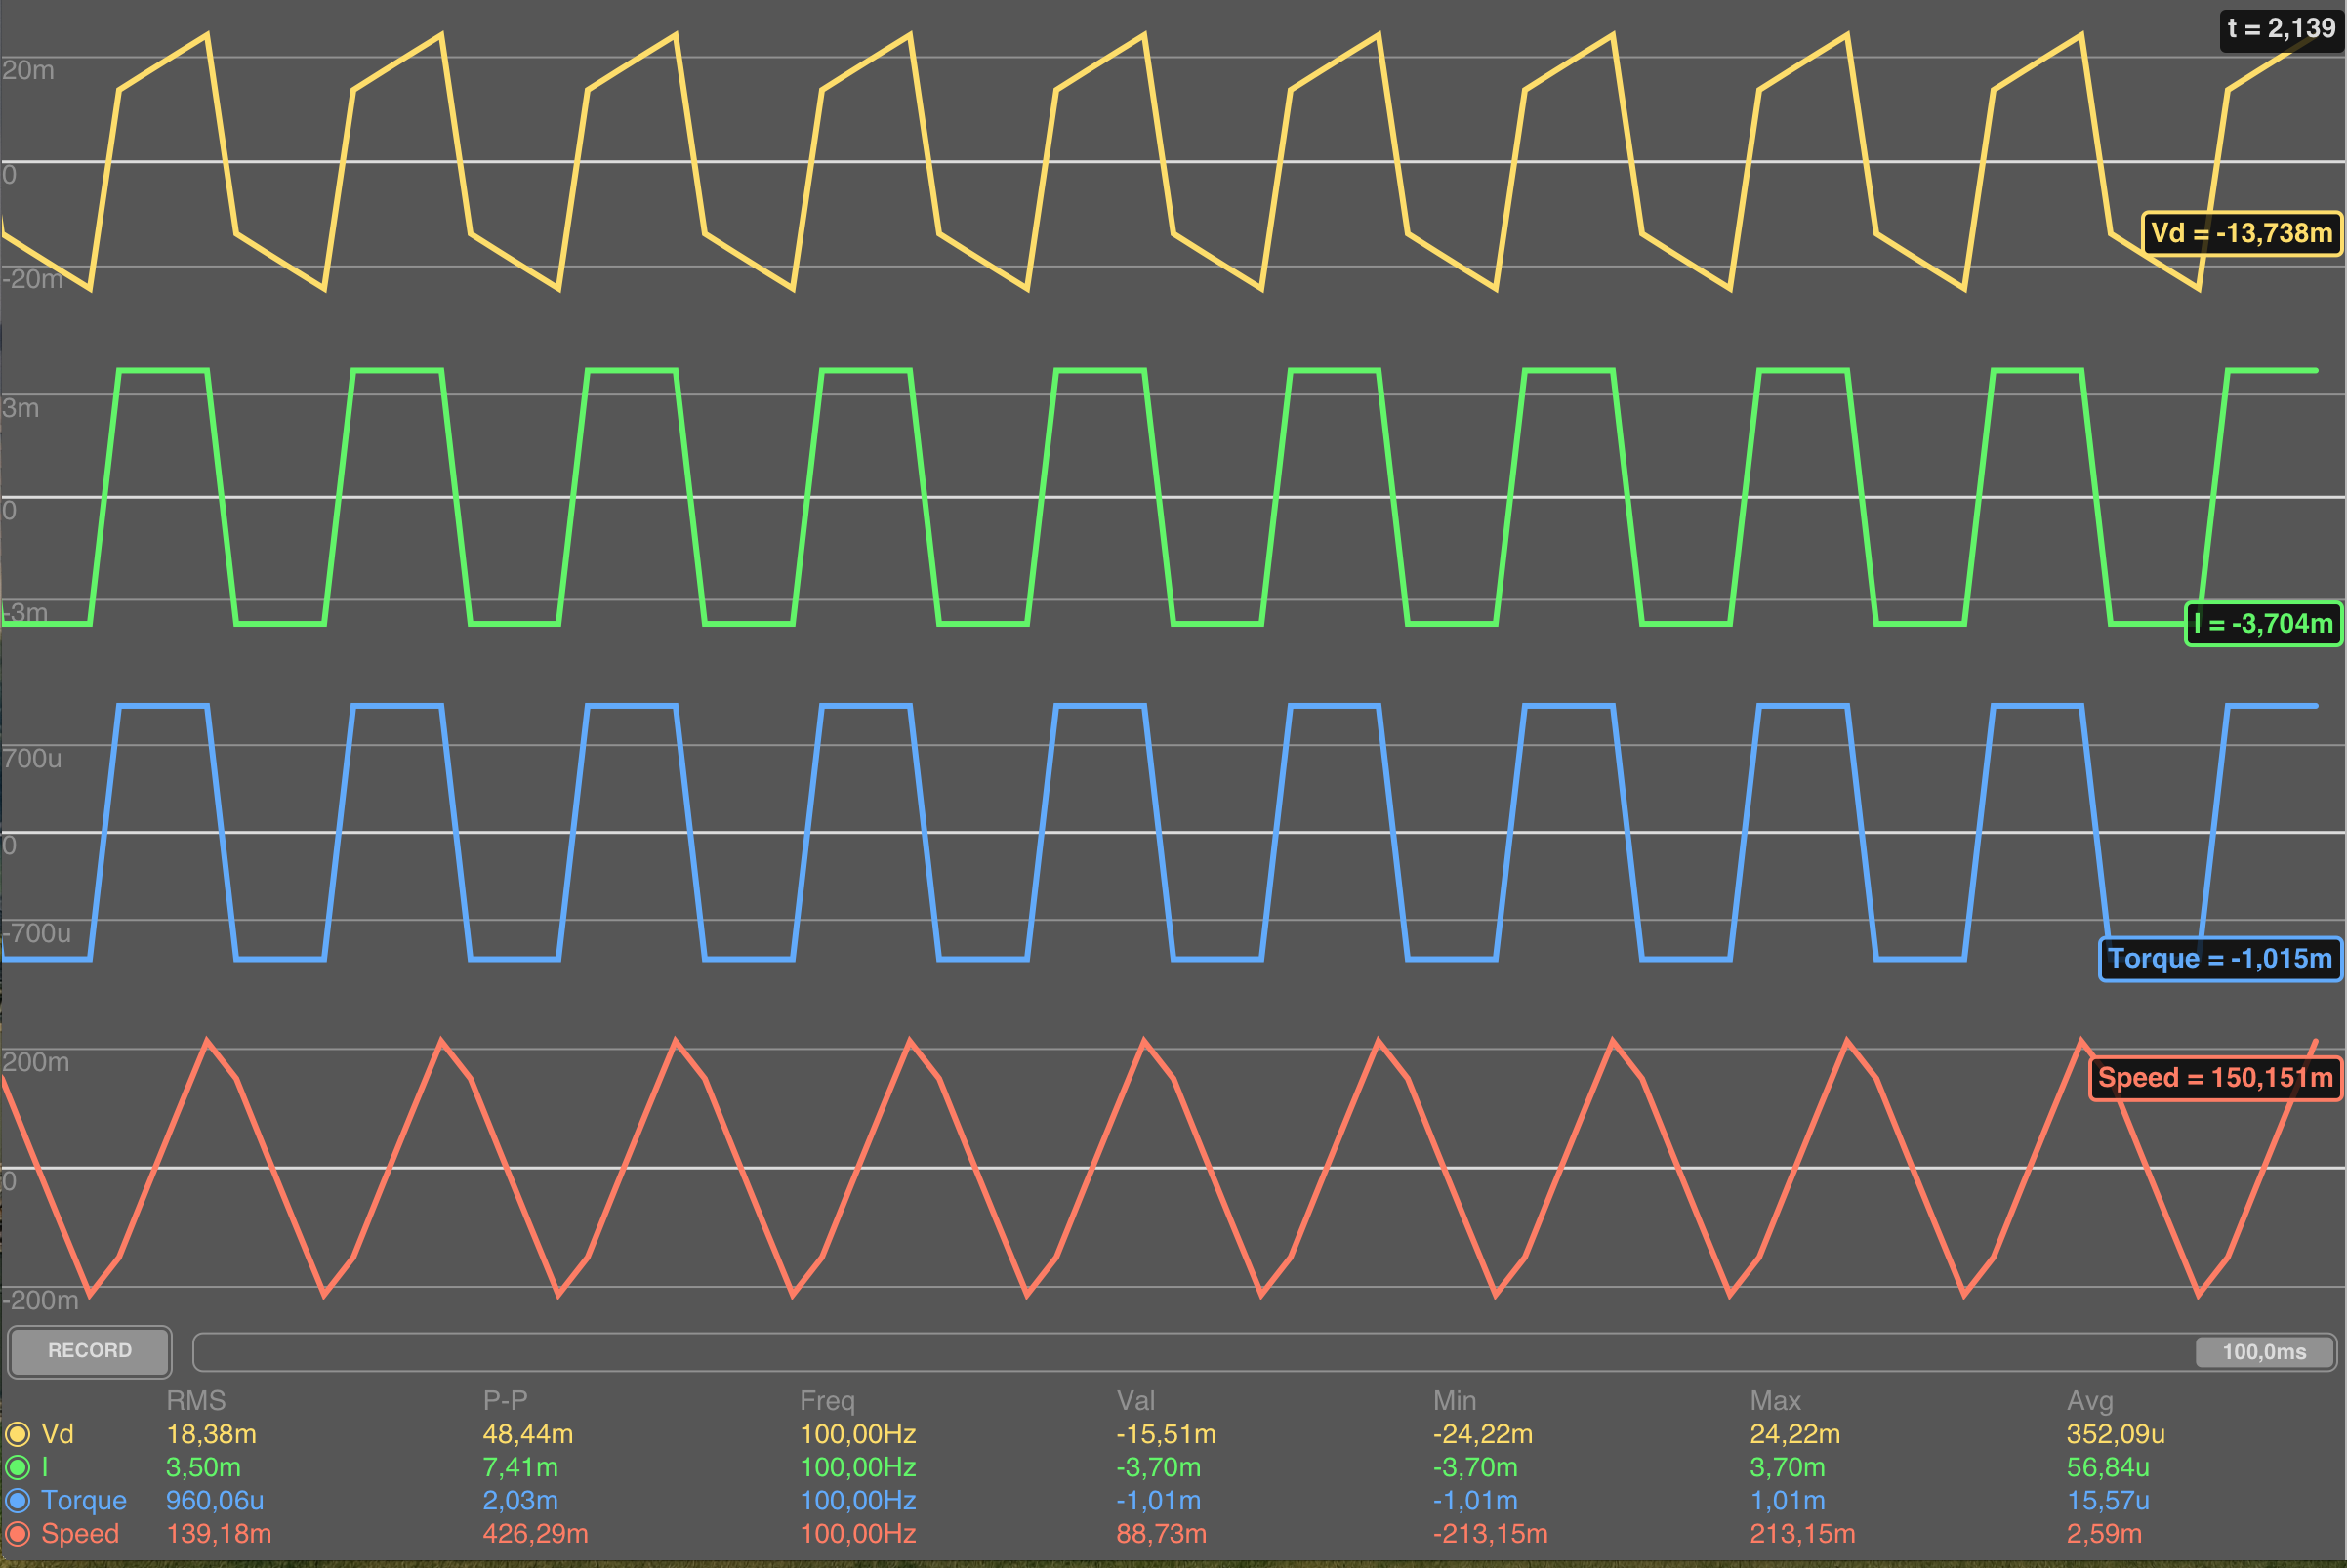
\includegraphics[width=1\textwidth]{simu0v}
	\caption{Simulation avec une commande de 0V}
\end{figure}
\begin{figure}
	\centering
	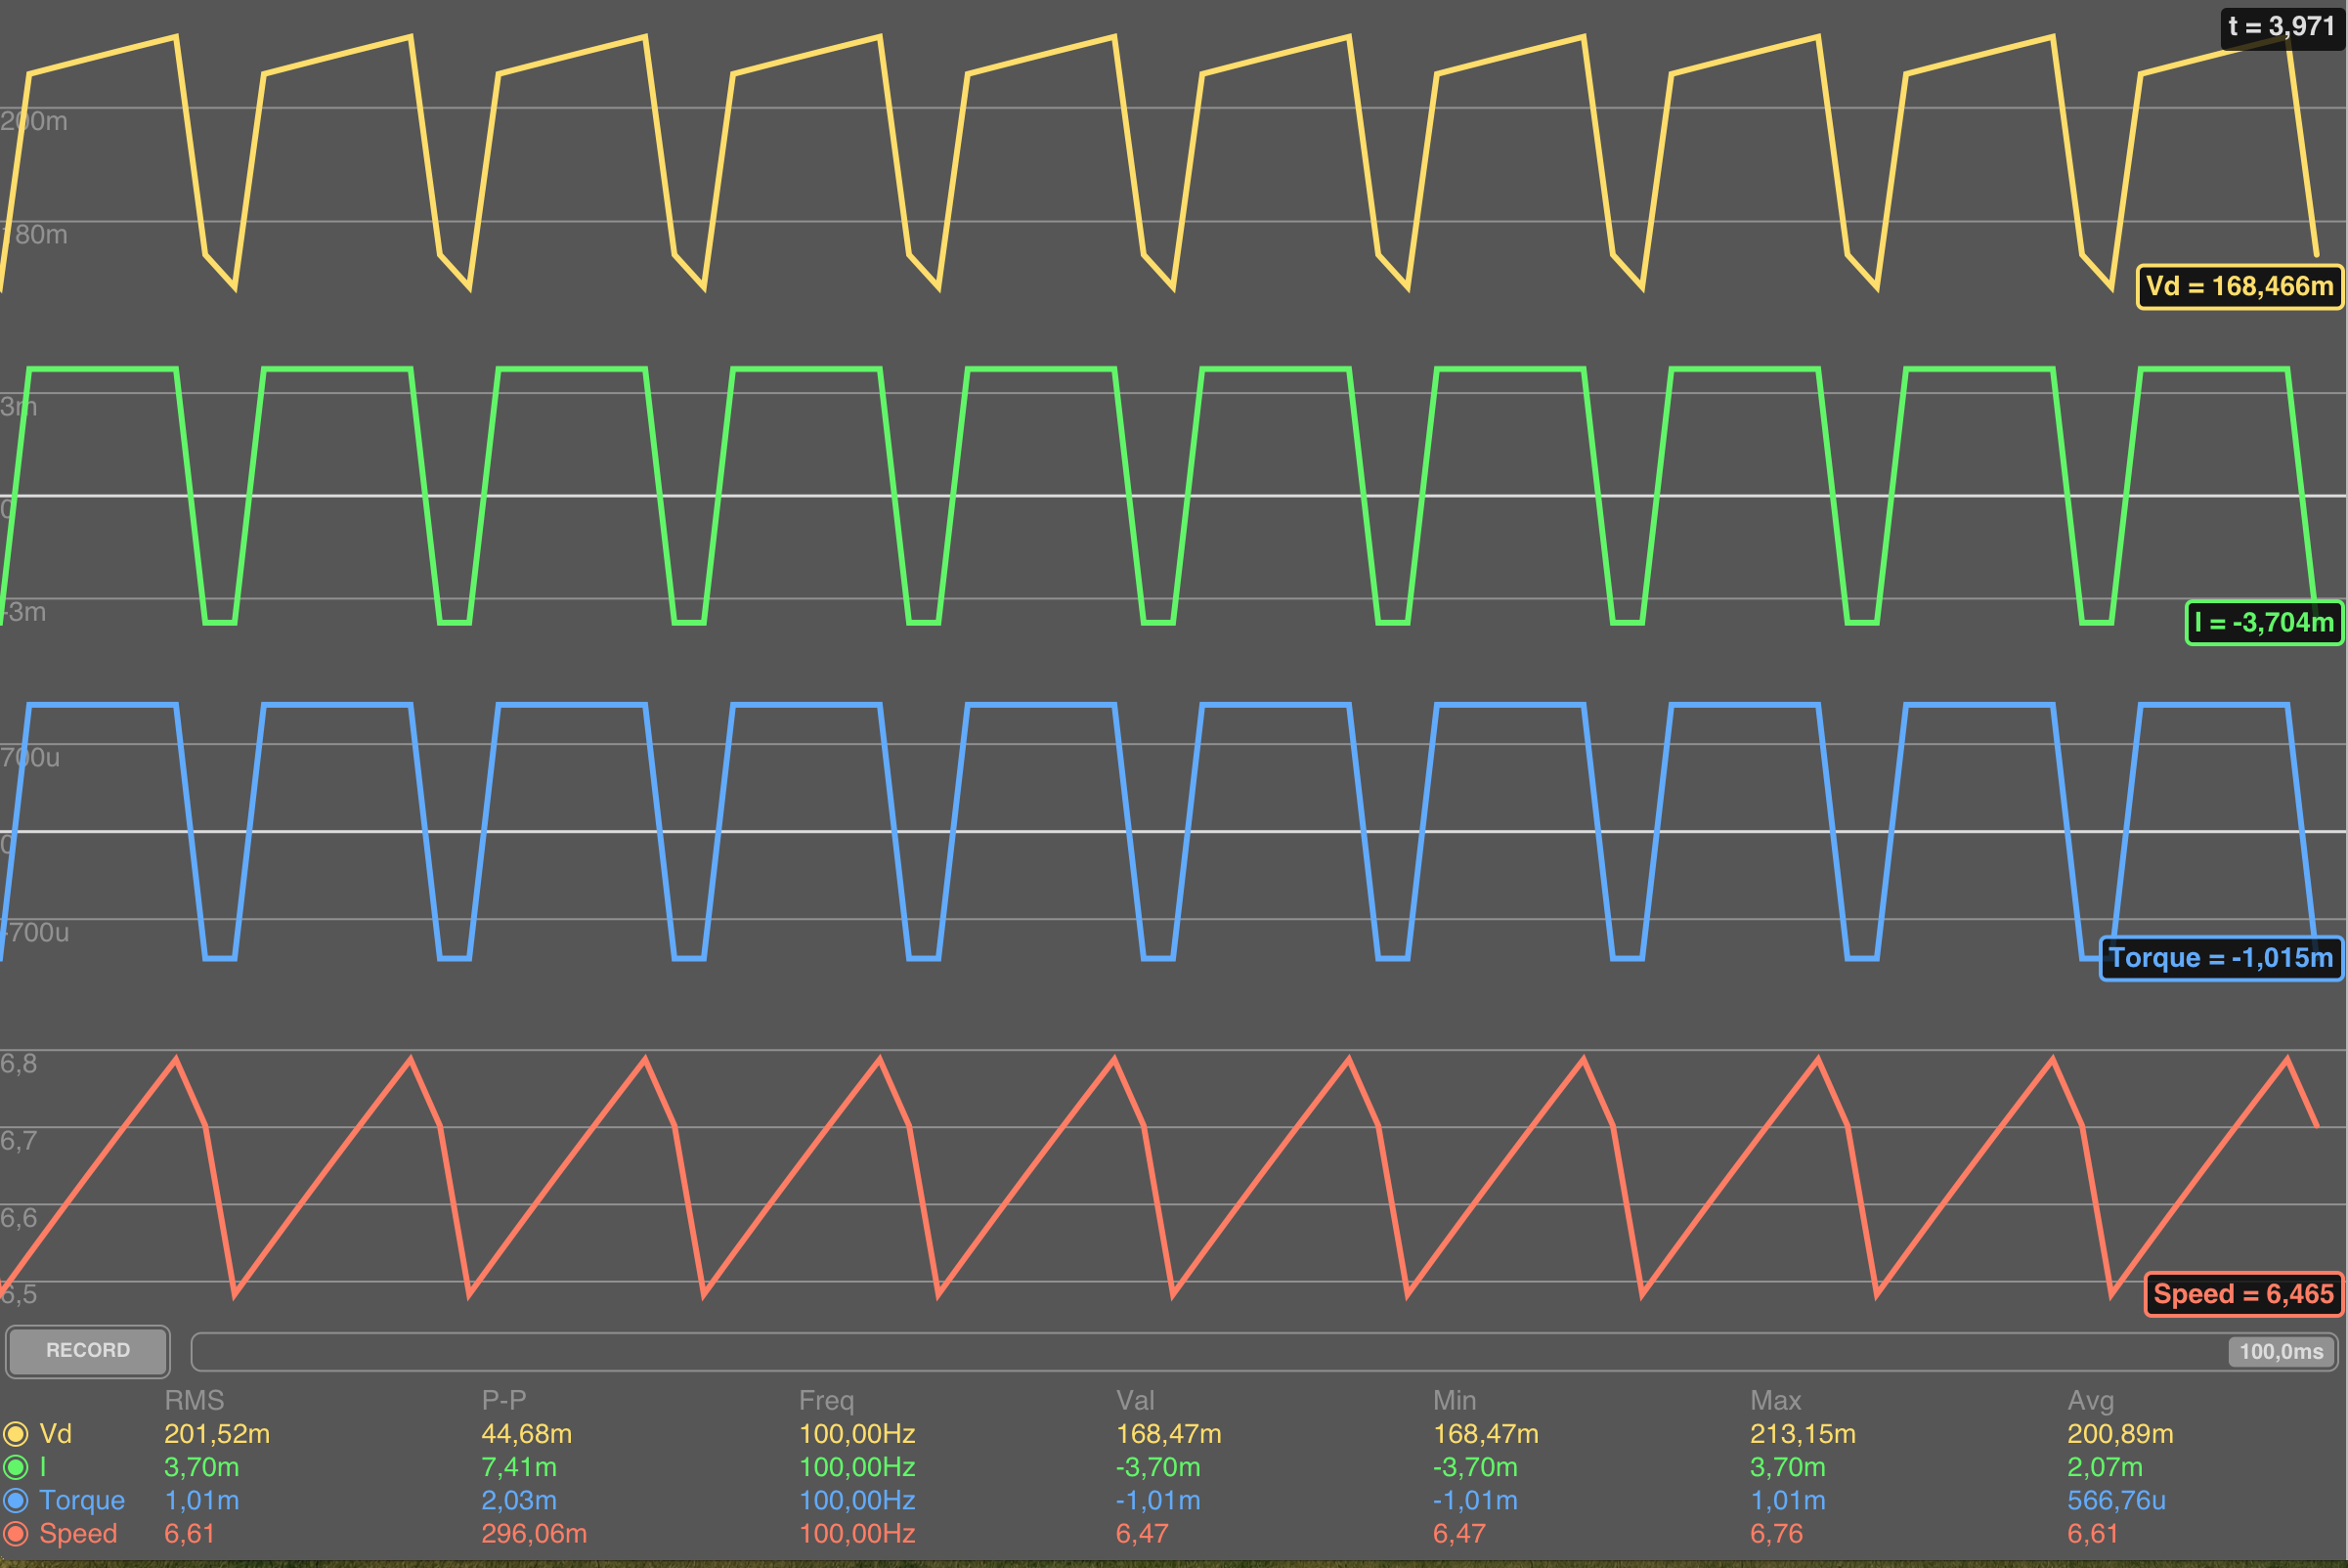
\includegraphics[width=1\textwidth]{simu7v}
	\caption{Simulation avec une commande de 7V}
\end{figure}
\begin{figure}
	\centering
	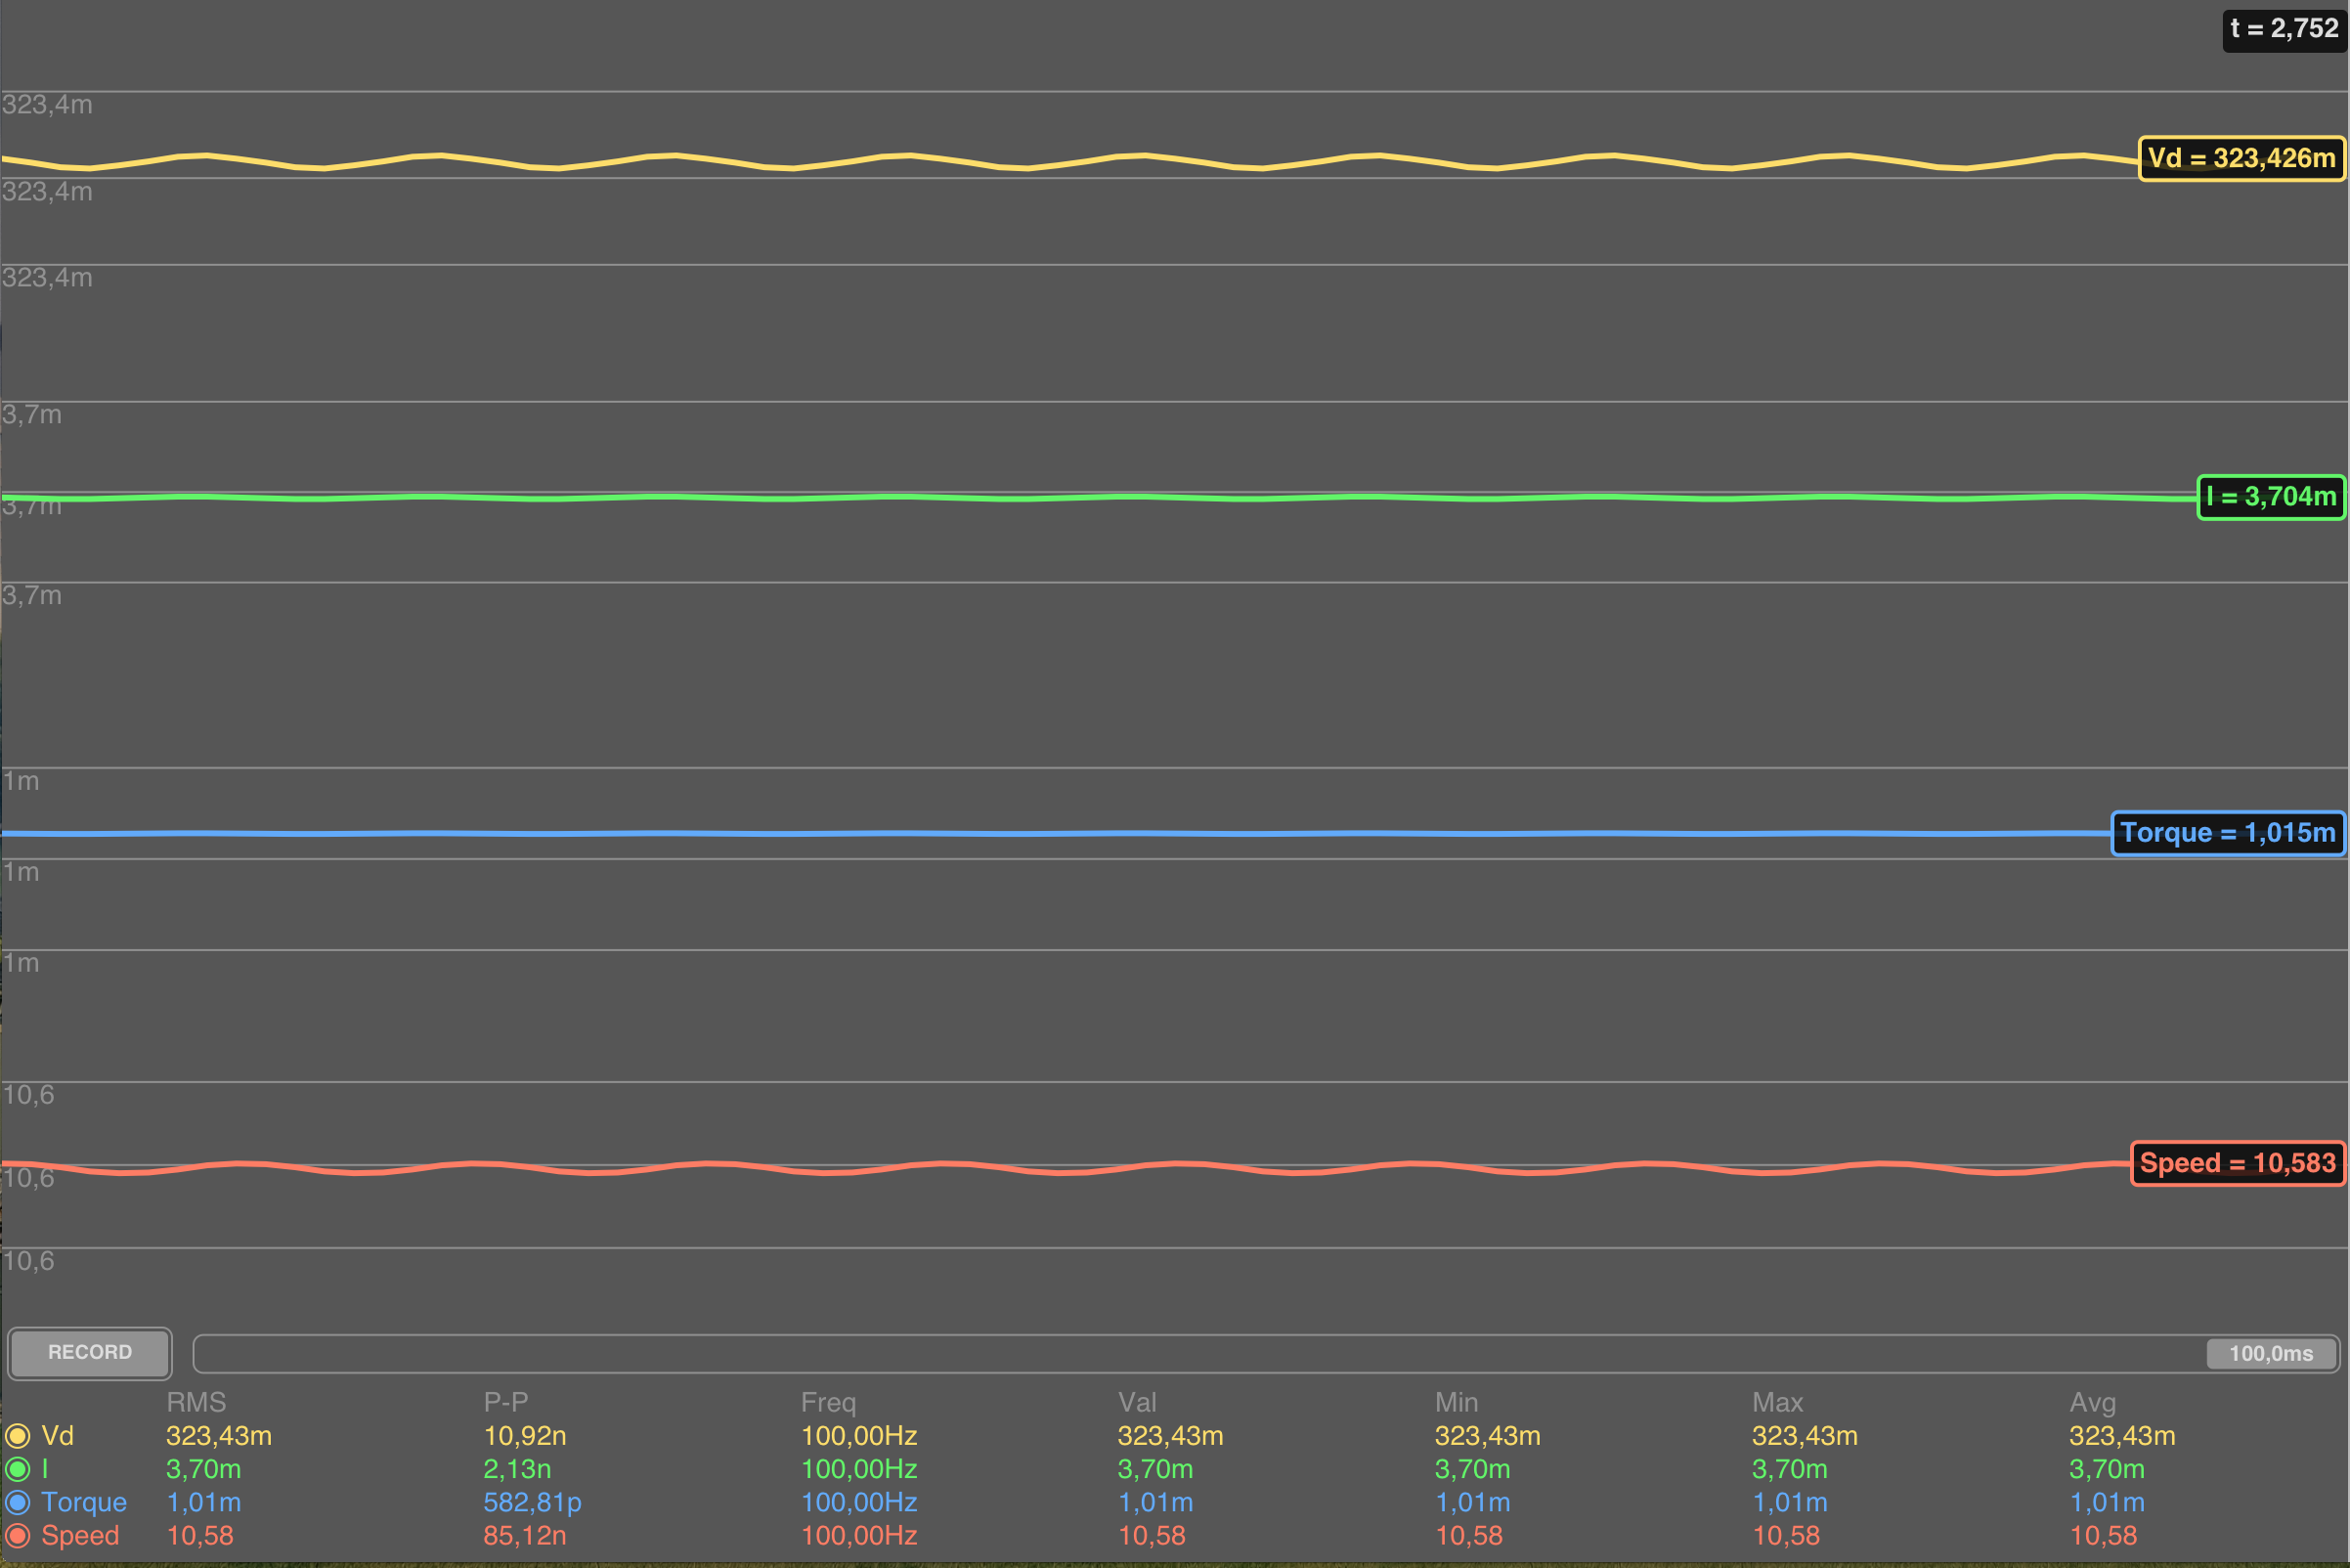
\includegraphics[width=1\textwidth]{simu15v}
	\caption{Simulation avec une commande de 15V}
\end{figure}


\subsection{Circuit}

\begin{figure}[h!]
  \centering
    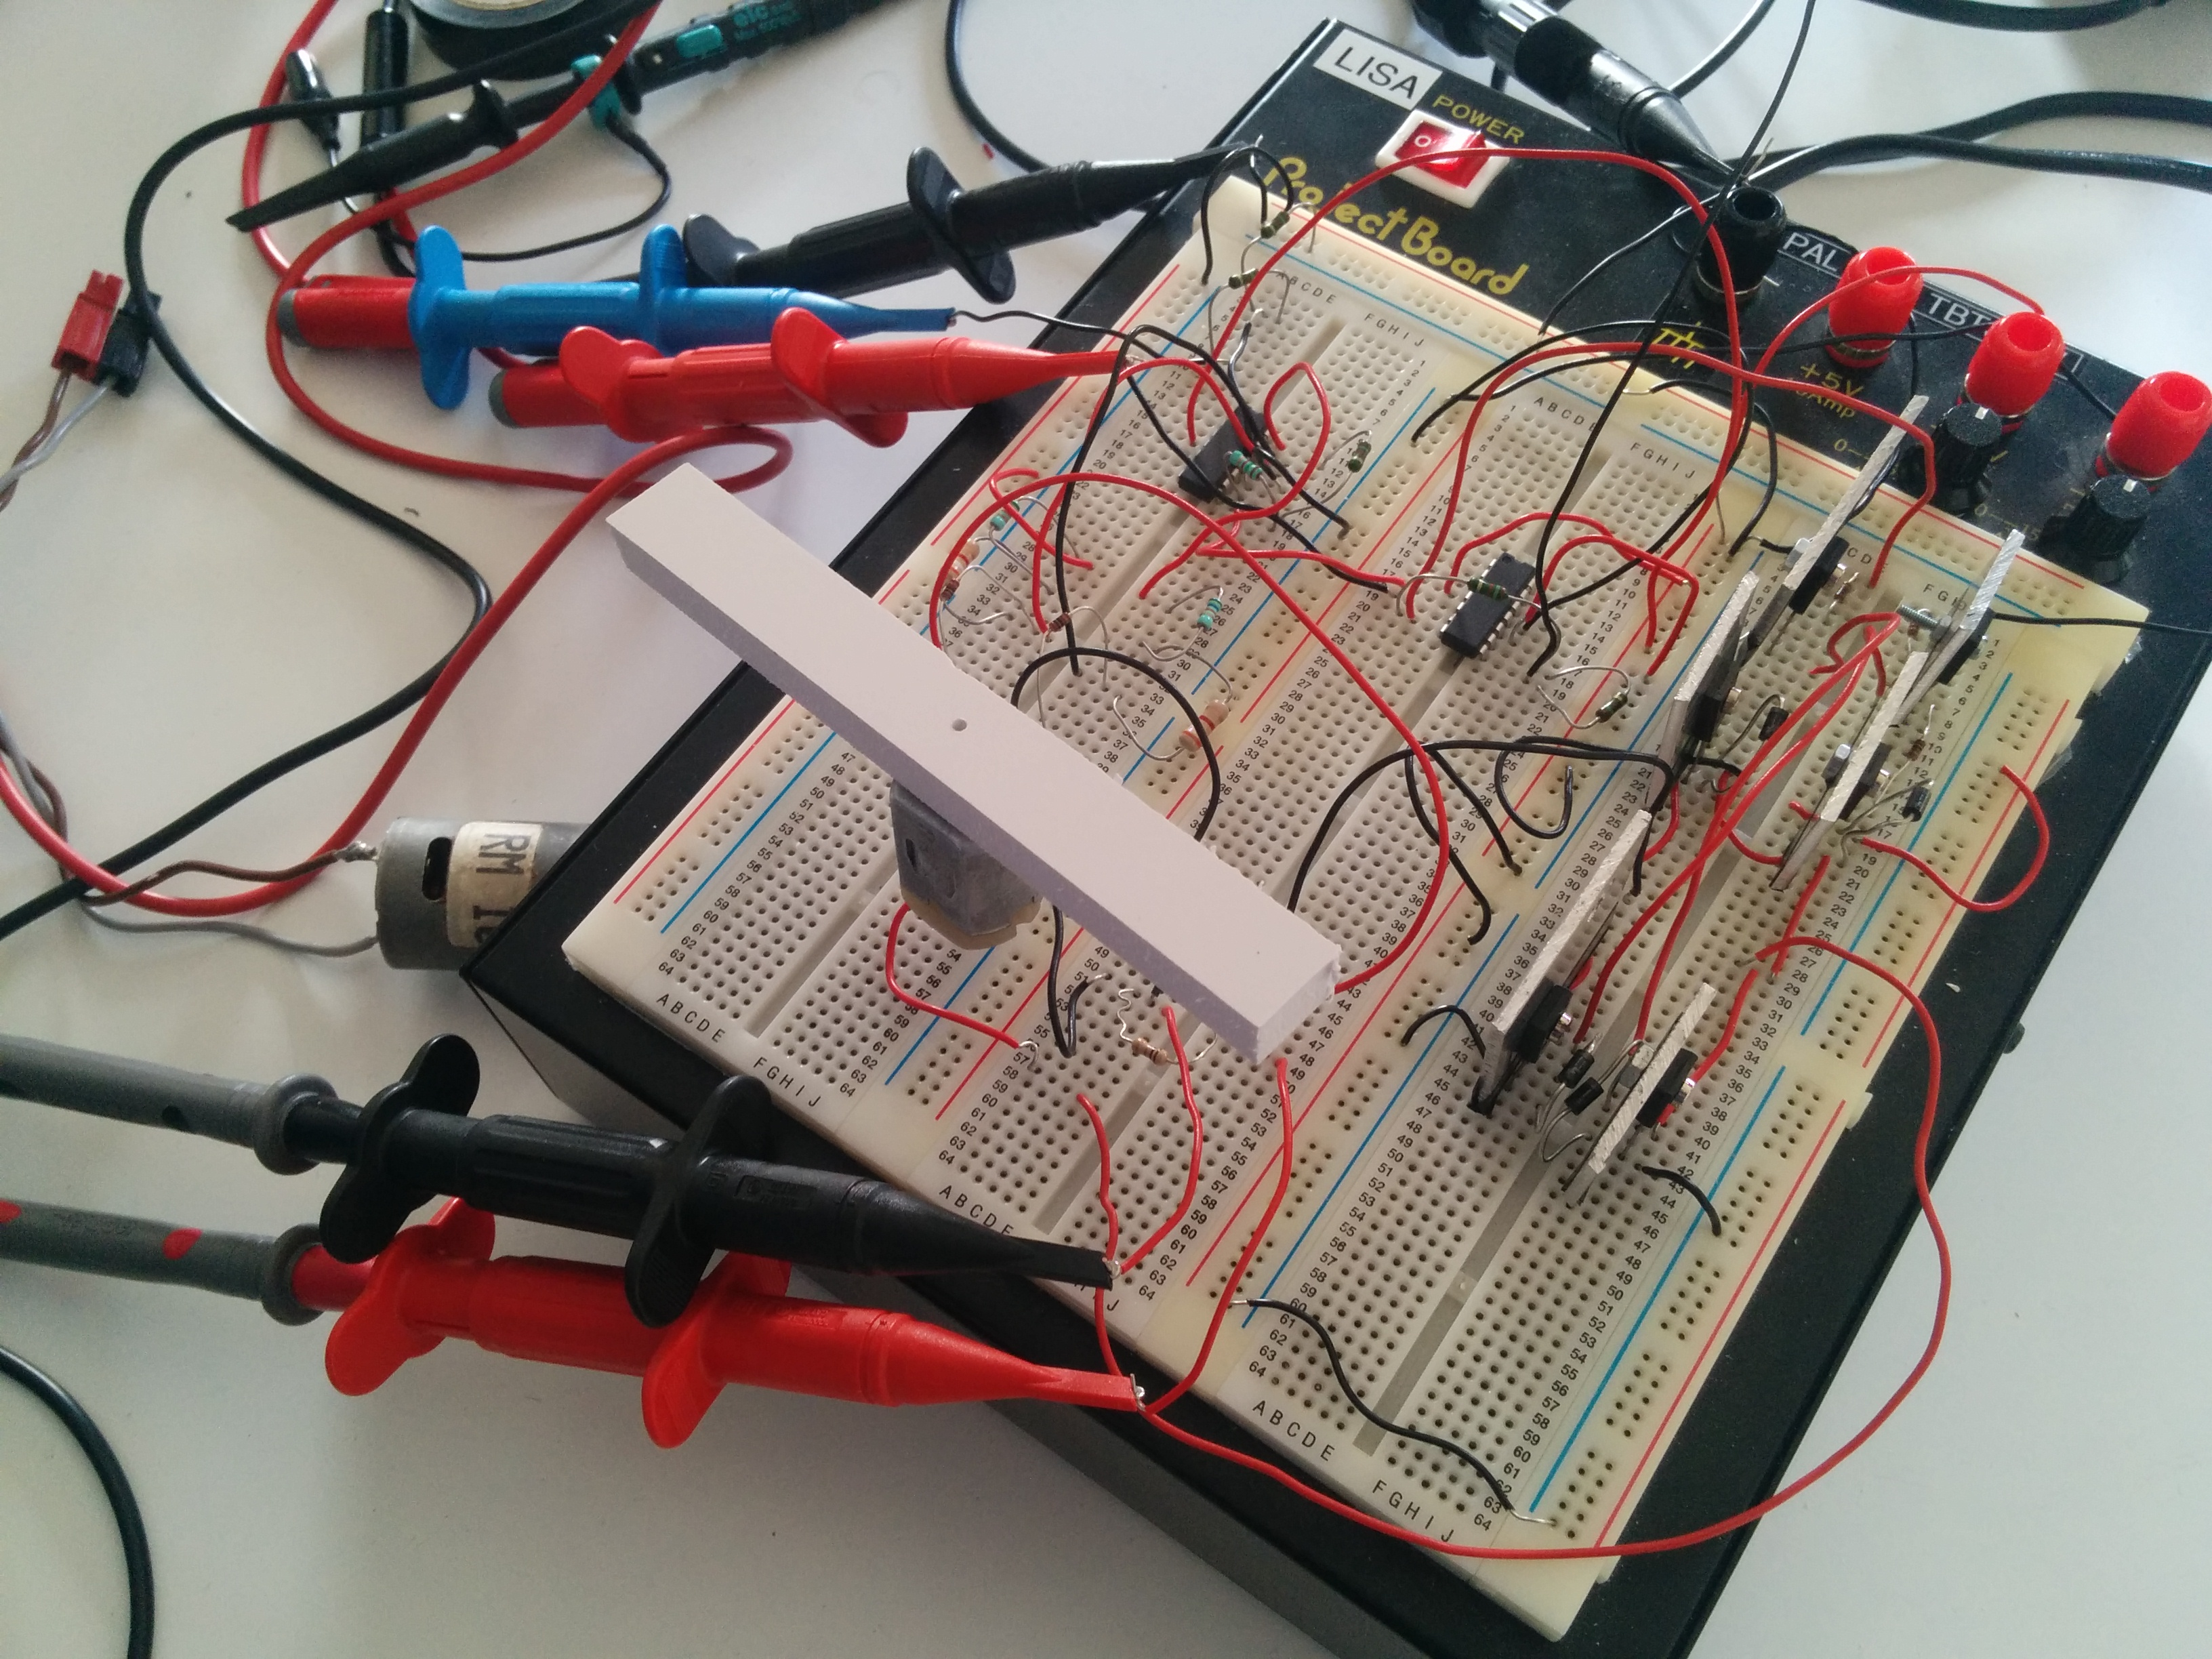
\includegraphics[width=1\textwidth]{circuit}
  \caption{Le circuit réalisé}
\end{figure}

\begin{figure}[h!]
  \centering
    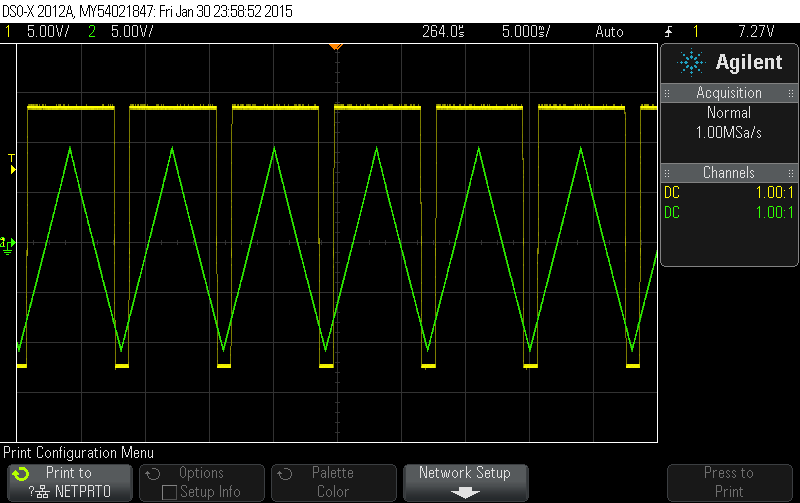
\includegraphics[width=1\textwidth]{scope_1}
  \caption{Entrée positive du pont en H}
\end{figure}

\begin{figure}[h!]
  \centering
    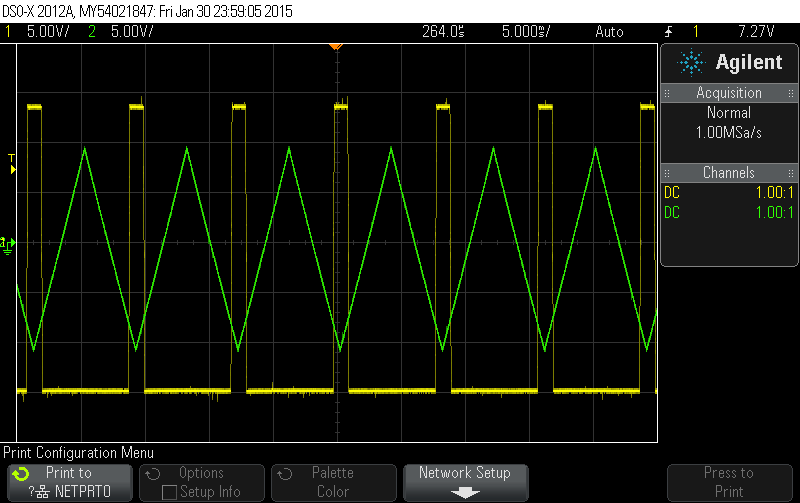
\includegraphics[width=1\textwidth]{scope_2}
  \caption{Entrée négative du pont en H}
\end{figure}

\begin{figure}[h!]
  \centering
    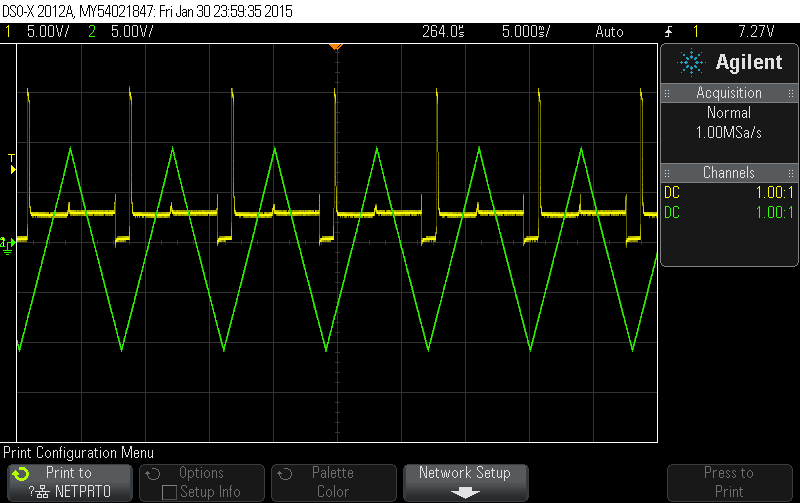
\includegraphics[width=1\textwidth]{scope_3}
  \caption{Tension aux bornes du moteur}
\end{figure}

\subsection{Résultats}

\section{Conclusion}

\end{document}